\documentclass[../../main.tex]{subfiles}

    \lstset{basicstyle=\small,
      showstringspaces=false,
      commentstyle=\color{black},
      keywordstyle=\color{blue}
    }

    \graphicspath{{images/Konzepte/}{../../images/Konzepte/}}


    \begin{document}
    \subsection{Elektronik Komponenten}
    In diesem Kapitel wird der Aufbau der Elektronik des Zuges beschrieben. Die Abbildung \ref{fig:et_komponenten} veranschaulicht den Aufbau der Elektronik. Darauf sind alle logischen Verbindungen eingezeichnet. Weitere elektrische Verbindungen für die Stromversorgung werden im Kapitel \ref{et_stromversorgung} erläutert.\\
    Zentral dabei ist der Mikrocontroller Tiny K22. Die Software auf dem Mikrocontroller initialisiert alle Komponenten, überwacht deren Status und sendet die nötigen Informationen an  das Pi. Diese Schnittstelle ist detailliert im Kapitel \ref{interface_pi_tiny} beschrieben.\\
    Die Schnittstelle über den Debugger zum PC wird hier nicht weiter beschrieben, da diese Verbindung nur zum Entwickeln benutzt wird und für das endgültige Produkt nicht mehr von Bedeutung ist.

    \begin{figure}[H]
        \centering
        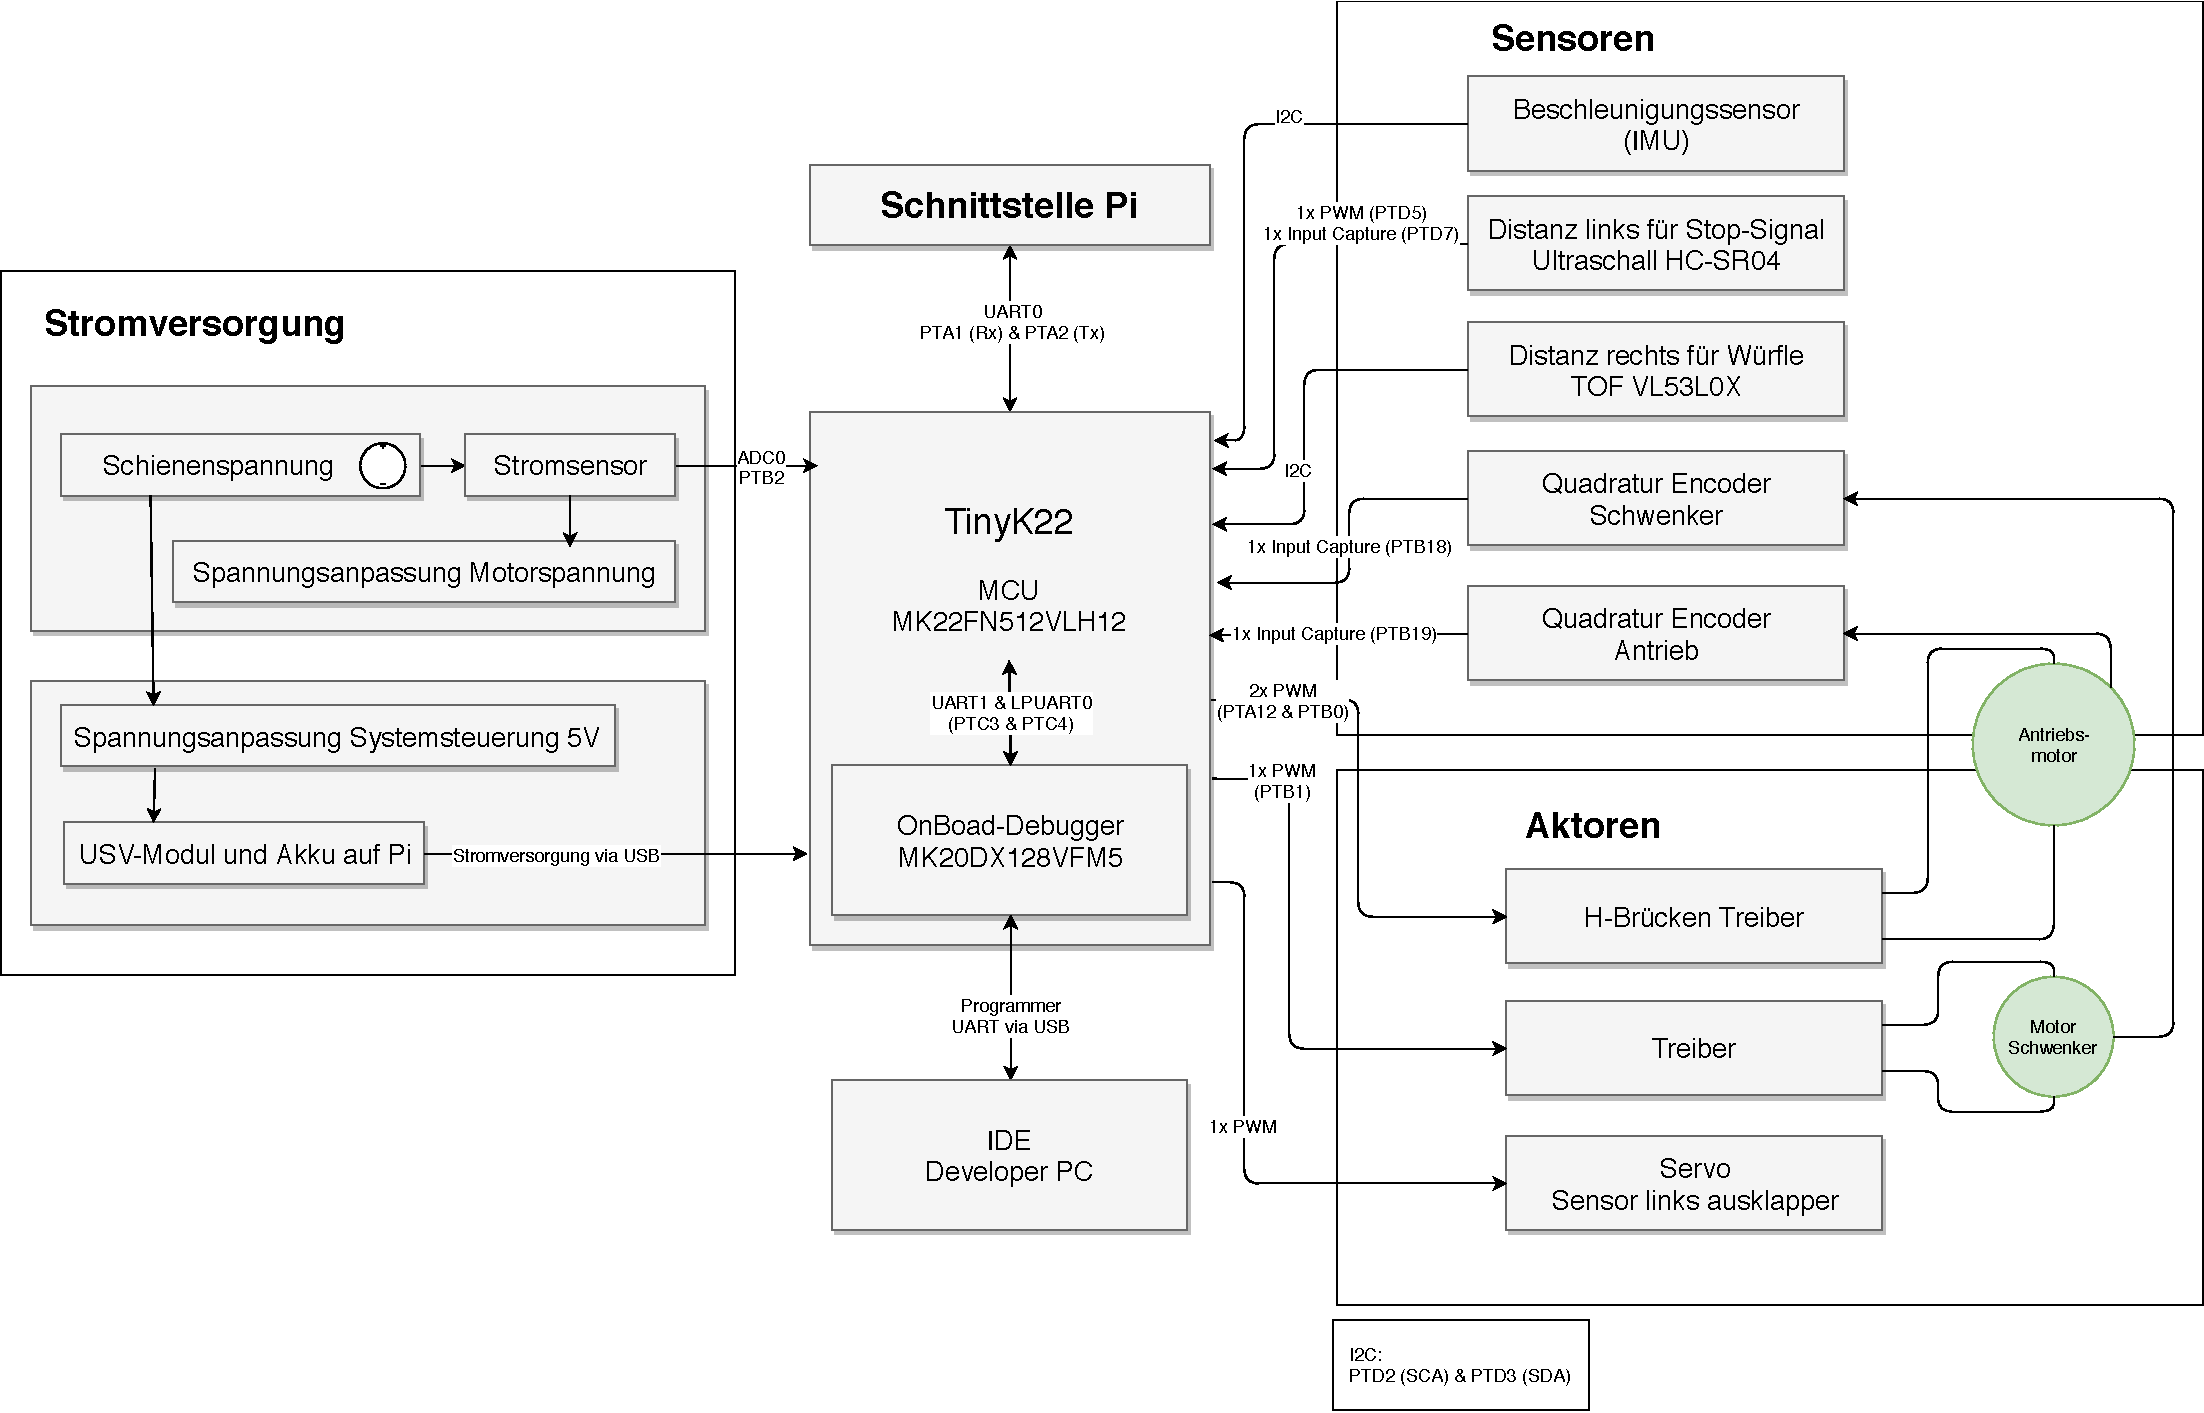
\includegraphics[width=1.0\textwidth]{../../drawings/KomponentenDiagramm/KomponentenDiagramm_ET.pdf}
        \caption {Komponentendiagramm Elektronik}
        \label{fig:et_komponenten}
    \end{figure}

    \subsubsection{Stromversorgung} \label{et_stromversorgung}
    Die Energie für das System wird über die Schienen bezogen. Die Antriebsenergie wird direkt von den Schienen bezogen und lediglich auf die korrekte Motorspannung angepasst. Die
    Systemsteuerung wird über ein StromPi 3 mit Strom versorgt. Als primäre Stromquelle wird dafür die Schienenspannung
    benutzt. Bei der Hochgeschwindigkeitsfahrt wird diese Quelle abgeschaltet, damit die gesamte Energie für den Antrieb
    zur Verfügung steht. Das StromPi schaltet automatisch auf die sekundäre Stromversorgung für das Pi um. Diese sekundäre
    Quelle wird durch einen LiFePO4-Akku auf dem StromPi realisiert. Sobald die primäre Stromquelle von den Schienen
    wieder zur Verfügung steht wird der Akku wieder nachgeladen.\\
    Das Pi zero und das TinyK22 mit diversen Sensoren und Aktoren werden über die USB-Anschlüsse des Pi versorgt.\\

    \textbf{Antriebsenergie}\\
    Die Energie für den Antrieb wird direkt von den Schienen bezogen. Bei der Hochgeschwindigkeitsfahrt werden alle anderen Verbraucher (z.B. Raspberry PI) von den Schienen entkoppelt, um die gesamte Energie für den Antrieb nutzen zu können.

    \textbf{Verpolungsschutz}\\
    Auf den Schienen steht eine Gleichspannung zur Verfügung, wobei eine Schienenseite der $+$ Pol und die andere Seite der $-$ Pol ist. Daraus ergibt sich das Problem, dass beim Platzieren des Zuges entgegen der vorgesehenen Fahrtrichtung eine Verpolung stattfindet. Auch ist die Zuordnung der Pole in der Aufgabenstellung noch nicht spezifiziert. Um sicherzustellen, dass das System unabhängig von der Polung der Schienen funktioniert, muss eine Gleichrichtung realisiert werden. Dies kann mit einem Brückengleichrichter realisiert werden. (siehe Abbildung \ref{fig:et_bruckengleichrichter})

    \begin{figure}[H]
        \centering
        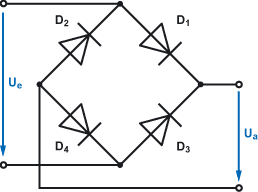
\includegraphics[width=0.3\textwidth]{Brueckengleichrichter.png}
        \caption {Brückengleichrichter (www.elektronik-kompendium.de)}
        \label{fig:et_bruckengleichrichter}
    \end{figure}

    Die Ausgangsspannung $U_a$ hat dabei immer dieselbe Polarität, unabhängig welche Polarität $U_e$ hat. \\
    Für den Hochgeschwindigkeitszug wird ein "B40C 3700-2200"  verwendet. Dabei handelt es sich um eine Integrierte Schaltung für einen Brückengleichrichter. Der maximal zulässige Strom ist dabei $3.7A$. Bei diesem Strom fällt über dem Gelichrichter eine Spannung von ca. $1V$ ab.

    \textbf{Spannungsanpassung}\\
    Gemäss der Aufgabenstellung stehen $20\pm2V$ bei bis zu $3A$ zur Verfügung. Aufgrund der grossen Toleranz von $4V$ muss die Spannung angepasst werden, um eine stabile Spannung sicherzustellen. Dafür wird ein DC-DC Converter verwendet. Dabei ist zu beachten, dass der Converter für den maximalen Strom von $3A$ ausgelegt ist.

    \textbf{Unterbrechungssicherheit}\\
    Um sicherzustellen, dass ein allfälliger Wackelkontakt der Schleifkontakte überbrückt werden kann und um grössere Spannungsschwankungen zu vermeiden, wird ein Kondensator zur Stützung eingesetzt.

    \textbf{Stromüberwachung}\\
    Um den Stromverbrauch des Antriebs zu überwachen, wird ein Strom Messwiderstand eingesetzt. Eine
    Differenzverstärker Schaltung bereitet die Spannung über dem Strom Messwiderstand auf, damit der Mikrocontroller mit
    dem Analog-Digital Wandler den Strom bestimmen kann. Mit dieser Information kann die Software des Mikrocontrollers
    auf Stromspitzen reagieren und z.B. die Geschwindigkeit reduzieren. Der Stromverbrauch ist auch für die Entwicklungs-
    und Testphase eine sehr wertvolle Information, damit das System optimal ausgelegt werden kann.
    Zur Messung wird ein "13FR200E - Strom Messwiderstand" verwendet. Dieser hat einen Widerstand von $0.2\Omega$. Der Strom kann daraus mit dem Ohmsches Gesetz bestimmt werden. $$I=\frac{U_R}{R}=\frac{U_R}{0.2\Omega} $$
    \\
    \textbf{Akku}\\
    Während der Hochgeschwindigkeitsfahrt wird die Systemsteuerung über einen Akku mit Storm versorgt. Die benötige Leistung der einzelnen Komponenten ist in Tabelle \ref{tab:et_komponente_leistung} aufgeführt. Im schlimmsten Fall soll der Akku das System dabei mindestens für zwei komplette Abläufe mit Energie versorgen können.\\
    Eine Runde darf maximal vier Minuten dauern. Das bedeutet die Energie des Akkus muss für mindestens acht Minuten reichen. Daraus ergibt sich für die Energie $$E=P\cdot t = 14.2W \cdot 8min = 113.6Wmin = 1.9Wh$$

    \begin{table}[H] \centering
        \begin{tabular}{|l|r|}
        \hline
        \textbf{Komponente}     & \textbf{Leistung (max)} \\ \hline
        Raspberry Pi 3 Model B  & 12.50W \nocite{PiShopPi3ModelBp}                 \\ \hline
        Raspberry Pi zero W     & 1.20W \nocite{RaspiTvPiZeroPower}                   \\ \hline
        Tiny K22                & 0.10W \nocite{K22DataSheet}       \\ \hline
        Encoder                 & 0.07W                   \\ \hline
        H-Brückentreiber        & 0.02W                   \\ \hline
        Treiber Schwenker Motor & 0.5mW                   \\ \hline
        Beschleunigungssensor   & 0.3mW                   \\ \hline
        TOF-Sensor              & 20mW                    \\ \hline
        Ultraschall Sensor      & 75mW                    \\ \hline
        \textbf{Total}          & \textbf{14.20W}         \\ \hline
        \end{tabular}
        \caption{benötigte Leistung der Komponenten}
        \label{tab:et_komponente_leistung}
    \end{table}

    Das StormPi Modul wird mit einem LiFePO4-Akku ergänzt. Der verbaute Akku hat $1000mAh$. Bei einer Spannung von $3.7V$ entspricht dies $3.7Wh$. \\
    Dies ist genügend für zwei Durchläufe. Ausserdem wird der Akku ausserhalb der Hochgeschwindigkeitsfahrt nachgeladen, was eine zusätzliche Reserve ergibt.

    \subsubsection{Sensoren} \label{et_sensoren}
    Mit diversen Sensoren sollen folgende Daten aufgenommen werden.
    \begin{itemize}
        \item Beschleunigung
        \item Geschwindigkeit
        \item Position
        \item Distanz rechts (für Erkennung Würfel)
        \item Distanz links (für Erkennung Haltesignal)
    \end{itemize}
    \pagebreak
    \textbf{Beschleunigung}\\
    Die Beschleunigung wird mit einem Beschleunigungssensor ADXL345 aufgenommen. Dieser kommuniziert über eine $I^2C$ Schnittstelle mit dem Mikrocontroller. Er liefert jeweils die Beschleunigung in x-, y-, und z-Richtung. Der Sensor wird parallel zur Fahrtrichtung montiert, so dass es genügt, eine Beschleunigungsrichtung für die Querbeschleunigung und eine Richtung für die Längsbeschleunigung auszuwerten. Die Verwendung des Sensors ist in Kapitel \ref{pi_beschleunigung} detailliert beschreiben.\\

    \textbf{Geschwindigkeit}\\
    Die Geschwindigkeit wird hauptsächlich über den Quadratur Encoder am Antriebsmotor aufgenommen. Zusätzlich wird die
    Geschwindigkeit über die Beschleunigung zur Kontrolle nachgerechnet.

    \paragraph{Quadratur Encoder:} Der Quadratur Encoder MR, Typ L gibt $1024$ Impulse pro Umdrehung. Der Verlauf eines Impulses ist in Abbildung \ref{fig:et_encoder} dargestellt. Der Encoder stellt drei Kanäle zur Verfügung. Über die Kanäle $A$ und $B$ kann einzeln die Geschwindigkeit bestimmt werden. Durch Auswerten der Phasenverschiebung der beiden Kanäle (''$A$ eilt $B$ vor'' oder ''$A$ eilt $B$ nach'') kann zusätzlich noch die Drehrichtung bestimmt werden. Der Kanal $I$ ist mit Kanal $A$ und $B$ synchronisiert und kann ebenfalls zur Bestimmung der Geschwindigkeit dienen.\\
    Für die Bestimmung der Geschwindigkeit kann die Dauer zwischen zwei Impulsen gemessen werden, oder es können die Anzahl Impulse in einer bestimmten Zeit gezählt werden. Für dieses Projekt soll die Dauer des Impulses gemessen werden. Der Vorteil dieser Methode ist die bessere Präzision, da nach jedem einzelnen Impuls die durchschnittliche Geschwindigkeit seit dem letzten Impuls sofort bestimmt werden kann. Das Risiko ist, dass bei hohen Umdrehungszahlen der Mikrocontroller nicht schnell genug ist mit dem Zählen, oder dass der Zähler des Mikrocontrollers bei sehr tiefen Umdrehungszahlen überläuft.\\
    Die maximale Umdrehungszahl des Antriebsmotors für die angestrebte Maximalgeschwindigkeit liegt bei $5200 min^{-1}$. Mit $1024$ Impulsen pro Umdrehung ergibt dies $$5200 min^{-1} \cdot 1024 Impulse = 5'324'800 \frac{Impulse}{min}$$
    Dies sind dann $$ 5'324'800 \frac{Impulse}{min} / 60s = 88'747 \frac{Impulse}{s} $$
    Dies ergibt eine Impulsdauer von $$\frac{1}{88'747 \frac{Impulse}{s}} = 11.29\mu s$$ Bei der schnellsten möglichen
    Timer-Einstellung auf dem TinyK22 ($60MHz$) ergibt dies noch $676 \frac{Ticks}{Impuls}$. Bei der Implementierung
    muss also beachtet werden, dass bei hoher Geschwindigkeit möglichst wenig Zeit in der Interrupt Routine verbracht
    wird, da diese dann sehr oft aufgerufen wird. Sollte sich zeigen, dass der Mikrocontrollers durch die hohe Impulsrate
    überlastet ist, muss ein Encoder mit weniger Impulsen pro Umdrehung gewählt werden oder ein Frequenz Teiler
    dazwischen geschaltet werden.\\
    Damit der Timer nicht überläuft, muss eine Impulsperiode fertig sein, bevor der Timer den Wert $$2^{32} \approx 4.29 Mrd$$ erreicht. Dies ergibt bei $60MHz$ eine Zeit von $$2^{32} \cdot \frac{1}{60MHz} = 71.58s$$ Also ist ein tiefstmögliche Umdrehungszahl $$\frac{1}{71.58s \cdot 1024} = 13.6 \cdot 10^{-6} s^{-1}$$
    Diese Umdrehungszahl sollte nicht unterschritten werden. Diese Zahl ist jedoch so klein, dass dies als Stillstand gewertet werden kann.

    \begin{figure}[H]
        \centering
        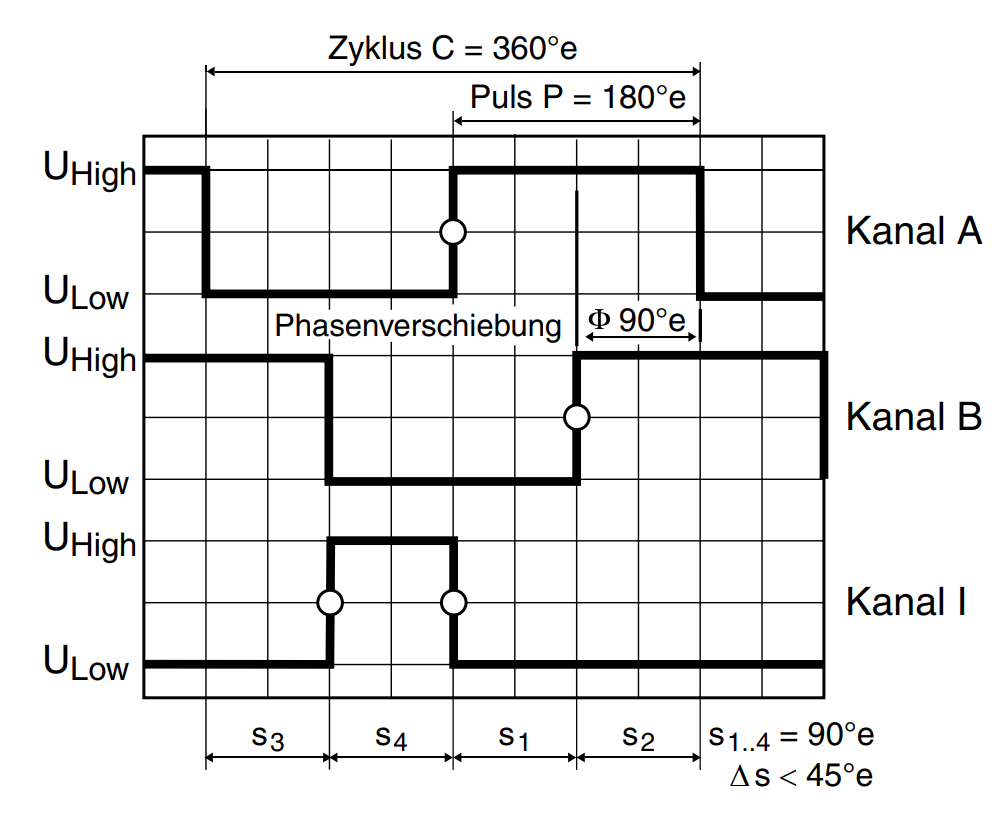
\includegraphics[width=0.6\textwidth]{Encoder_MR.png}
        \caption {Signalverlauf Encoder (www.maxonmotor.ch)}
        \label{fig:et_encoder}
    \end{figure}

    Die Geschwindigkeit des Zuges ($v_{Zug}$) kann somit aus der Umdrehungszahl des Motors ($N_{Motor}$) mittels der Mechanischen Übersetzung und der Grösse der Räder berechnet werden.
    $$v_{Zug}(N_{Motor}) = \frac{N_{Motor}}{2} \cdot d \cdot \pi$$\\
    $d:$ Raddurchmesser $22mm$\\

    \paragraph{Nachrechnen der Geschwindigkeit:}
    Unter der Annahme, dass zu Beginn der Messung zum Zeitpunkt $t = 0$ die Geschwindigkeit $0$ ist $(v(t=0) = 0)$, kann die Geschwindigkeit zum Zeitpunkt $t$ bestimmt werden mit $$v(t) = \int_{0}^{t} a(x) dx$$.\\
    Da aber auf einem Digitalen System die Daten nur zu diskreten Zeitpunkten ausgewertet werden können, ergibt sich dann eine Summen der Beschleunigungen zum Zeitpunkt $k$ $$v[k] = \sum_{i=0}^{k}a[i] \Delta t$$

    \textbf{Position}\\
    Über den Beschleunigungssensor kann man die aktuelle Position auf der Fahrbahn berechnen. Die zurückgelegte Strecke errechnet sich durch Integration der Geschwindigkeit oder durch zweifache Integration der Beschleunigung.\\
    Unter der Annahme, dass zu Beginn der Messung zum Zeitpunkt $t = 0$ die zurückgelegte Strecke $0$ ist $(s(t=0) = 0)$, kann die Geschwindigkeit zum Zeitpunkt $t$ bestimmt werden mit $$s(t) = \int_{0}^{t} v(x) dx$$\\
    Da aber auf einem Digitalen System die Daten nur zu diskreten Zeitpunkten ausgewertet werden können, ergibt sich dann eine Summen der Geschwindigkeiten zum Zeitpunkt $k$ $$s[k] = \sum_{i=0}^{k}v[i] \Delta t$$\\
    Die Geschwindigkeit wird gemäss der Beschreibung oben bestimmt.

    \textbf{Distanz}\\
    Auf beiden Seiten des Zuges wird eine Distanzmessung benötigt. Auf der rechten Seite des Zuges muss der Würfel erkannt werden, und auf der linken Seite soll ein ausklappbarer Sensor am Schluss die genaue Distanz zum Haltesignal bestimmen.

    \paragraph{Würfelerkennung:}
    Gemäss der Aufgabenstellung befindet sich der Würfel in einem Abstand von $8\pm1cm$ von der Gleismitte. Somit muss der Distanzsensor Distanzen zwischen ca. $20mm$ und $80mm$ erkennen können. Der exakte Wert der Distanz ist dabei nicht entscheidend, da nur ein bestimmter Schwellwert erkannt werden muss. Die Distanz zum Würfel wird mit einem TOF (Timo-Of-Flight) Sensor VL53L0X ermittelt.

    \paragraph{Haltesignal Erkennung:}
    Um möglichst präzise anhalten zu können, muss die Systemsteuerung den exakten Wert der Distanz zum Haltesignal kennen. Dies wird mit einem Distanzsensor ermittelt. Diese Distanz wird mit einem Ultraschall Sensor HC-SR04 gemessen. Es ist entscheidend, dass der Sensor korrekt und mit wenig Toleranz auf der Mechanik befestigt wird, um eine exakte Ausrichtung auf das Haltesignal sicherzustellen.

    \subsubsection{Aktoren}
    Die Aktoren stellen die Schnittstelle zur Mechanik dar. Diese sollen alle nötigen mechanischen Bewegungen auf Befehl des Mikrocontrollers ausführen.\\

    \textbf{H-Brücken Treiber für Antriebsmotor}\\
    Um den Antriebsmotor anzusteuern, wird ein H-Brückentreiber verwendet. Damit kann der Motor durch ein PWM Signal in der Geschwindigkeit fast beliebig eingestellt werden. Über die wahlweise Ansteuerung einer der beiden Eingänge der H-Brücke wird die Richtung bestimmt.\\
    Es wird ein Arduion IBT\_2 DC-Motoren Treiber mit einem BTS7960 eingesetzt. Dieses Bauteil kann Motoren mit einem Strom von bis zu 43A versorgen. \\

    \textbf{Antriebsmotor}\\
    Als Antriebsmotor dient ein Maxon DCX 32 L. Dieser kann eine Leistung von bis zu 70 Watt umsetzen. Dabei zu beachten ist, dass der Anlaufstrom bis zu $70A$ betragen kann. Dieser Strom muss begrenzt werden, indem der Mikrocontroller die Beschleunigung gemäss dem gemessenen Stromverbrauch anpasst. \cite{MaxonDCX32L} Dies ist bei einer Versorgungsspannung von 24V spezifiziert. Da aber nicht die maximale Drehzahl benötigt wird, kann auch eine entsprechend tiefere Spannung angelegt werden. Die Drehzahlkonstante des Motors ist $350 \frac{min^{-1}}{V}$. Für die angestrebte Drehzahl von $5200min^{-1}$ ergibt sich eine Spannung von $$\frac{5200min^{-1}}{350 \frac{min^{-1}}{V}} =14.8V$$ Somit muss der Antriebsmotor mit einer Spannung von mindestens $14.8V$ versorgt werden.\\

    \textbf{Motortreiber für Schwenker-Motor}\\
    Da die Richtung immer dieselbe ist reicht für den Schwenker ein normaler DC-Motoren Treiber. Um eine sanfte Beschleunigung und Bremsung der Konstruktion zu ermöglichen, soll auch der Schwenker-Motor mit einem PWM angesteuert werden. Als Treiber wird ein Board mit einem L298N verwendet.\\

    \textbf{Schwenker-Motor}\\
    Für den Schwenker wird ein Maxon DCX 19 S verwendet. Um die Position des Schwenkers zu bestimmen, ist auch an diesem Motor ein Encoder befestigt. Durch die Bestimmung der nötigen Umdrehungen, bis der Schwenker eingefahren ist, kann genau festgestellt werden, wie viele Impulse abgewartet werden müssen, bis der Motor anhalten muss. \cite{MaxonDCX19S}\\

    \textbf{Distanzsensor links ausklappen}\\
    Um den Sensor beim Parkieren ausklappen zu können, wird dieser an einem Servo befestigt. Sobald die Systemsteuerung entscheidet, dass das korrekte Haltesignal das Nächste ist, gibt sie den Befehl den Sensor auszuklappen. Dafür wird ein "Tower Pro Micro Servo SG90" verwendet. Dieser hat ein Drehmoment von bis zu $2.5 kg-cm$. \cite{SG90Datasheet}\\

    \subsubsection{Proof-of-Concept}
    Um die Funktionsfähigkeit der einzelnen Komponenten sicherzustellen, wurden diverse Tests gemacht. Das Ziel dieser Tests war es, die einfachste Form jeder Funktionalität zu realisieren. Auf eine quantitativ genaue Anpassung wurde in diesem ersten Schritt verzichtet, dies ist für die Realisierung des Projekts vorgesehen. Das Ziel der Tests war somit nur, zu zeigen, dass die Komponente wie vorgesehen funktionnieren kann. Eine Übersicht der durchgeführten Tests ist in Tabelle \ref{tab:poc_et} ersichtlich.\\

    \begin{table}[H]
        \centering
        \begin{tabular}{|l|p{10cm}|r|}
        \hline
        \textbf{Komponente}   & \textbf{Beschreibung des Tests}                                                                                                                                                                                                                                                                                                                  & \textbf{Ok} \\ \hline
        Tiny K22              & Der Mikrocontroller konnte erfolgreich programmiert werden und Hardware kann darüber angesteuert werden.                                                                                                                                                                                                                                         & \checkmark       \\ \hline
        UART Kommunikation    & Mittels dem "Raspberry Pi APROG HAT" konnte erfolgreich zwischen dem Pi und dem Tiny mittels UART kommuniziert werden.                                                                                                                                                                                                                           & \checkmark       \\ \hline
        Beschleunigungssensor & Der Beschleunigungssensor wurde über die Schnittstelle angesteuert und die Werte für die x-, y- und z-Richtung konnten erfolgreich ausgelesen werden.                                                                                                                                                                                            & \checkmark       \\ \hline
        Motorenansteuerung    & Vom Mikrocontroller wurde ein PWM generiert. Der Pin mit dem PWM wurde mit dem Motorentreiber Arduion IBT 2 und dieser dann mit einem Motor verbunden. Durch Vorgaben des Mikrocontrollers konnte die Geschwindigkeit und die Richtung des Motors eingestellt werden.                                                                            & \checkmark       \\ \hline
        Encoder               & Der Encoder wurde vom Mikrocontroller ausgelesen und die Zeiten und Impulse ausgewertet. Es zeigte sich, dass der Encoder korrekt 1024 Impulse pro Umdrehung liefert. Daraus lies sich dann die Umdrehungszahl berechnen. Auch wurde eine Zeitmessung durchgeführt, um festzustellen wie viel Zeit die Interrupt-Routine von der Flanke des Encoders, bis die Routine beendet ist benötigt. Hochgerechnet für die maximale Geschwindigkeit ergibt dies eine Auslastung des Mikrocontrollers von ca. 10\%.                                                                                                                        & \checkmark       \\ \hline
        Ultraschallsensor     & Der Ultraschallsensor wurde vom Mikrocontroller gemäss dem Datenblatt angesteuert. Mittels der gemessenen Zeit konnte eine approximative Distanz berechnet werden. Für einen exakten Wert sind noch genauere Abstimmungen nötig. Der Sensor reagiert jedoch zuverlässig auf Objekte in der Grösse des Würfels oder der Haltesignale.             & \checkmark       \\ \hline
        TOF-Sensor            & Mit einer Code-Bibliothek, die für das Tiny K22 angepasst wurde, konnte der TOF-Sensor erfolgreich angesteuert werden. Damit kann eine approximative Distanz berechnet werden. Für einen exakten Wert sind noch genauere Abstimmungen nötig. Der Sensor reagiert jedoch zuverlässig auf Objekte in der Grösse des Würfels oder der Haltesignale. & \checkmark       \\ \hline
        Spannungsanpassung    & Der DC-DC Converter wurde mit einer Spannungsquelle verbunden und die Ausgangsspannung bei diversen Einstellungen korrekt gemessen.                                                                                                                                                                                                              & \checkmark       \\ \hline
        Stromüberwachung      & Eine Differenzverstärker Schaltung wurde mit unterschiedlichen Lastwiderständen simuliert und durch die Messspannung den Strom bestimmt und mit dem Strom der Simulation verglichen.                                                                                                                                                             & \checkmark       \\ \hline
        \end{tabular}
        \caption{Übersicht Proof-of-Concept Elektronik}
        \label{tab:poc_et}
        \end{table}

    \end{document}